\part{Tensor Networks and Entanglement Invariants} 
\label{sec:qubit-invariants}

It is typical to consider a symmetry of a density operator $\rho$ or state $\psi$ as an operator satisfying 
\be 
\rho = V\rho V^\dagger
\ee 
\be 
\psi = M \psi
\ee
and so one could say that $\rho$ is invariant under $V$ and $\psi$ is
invariant under $M$ --- see Example \ref{ex:group-sym}.
If the relations holds for all elements of a matrix group, then we say
that $\rho$ or $\psi$ are invariant under the left multiplicative action of the group.
There are more subtle symmetries however.  
These are formed by considering polynomials in the coefficients of $\rho$ or $\psi$ that are left invariant under the action of a group.  The study of such polynomials is known as 
Invariant Theory \cite{hilbert}.  David Hilbert made notable progress on the topic of invariant theory, which he perused throughout his life.  There has been past work on considering these invariants in the context of quantum information science.  Some of our personal favorites include \cite{entinv2, entinv3, entinv1} as well as some work more closely related to this chapter \cite{BBL11}. Algebraic geometry has also been applied to tensor networks in \cite{2014SIGMA..10..095C}. 

\begin{example}[Group Symmetry of $\rho$]\label{ex:group-sym}
 We will consider a general density operator $\rho$ and look for $V\in U(d)$ such that 
 \be 
 \rho = V\rho V^\dagger
 \ee 
 this implies that $[\rho, V]=0$ and we arrive at a basis for $G$ by noting the unitary operators that commute with $\rho$.  
 That is, $\{\ket{\lambda_i}\}_i$ such that $\rho = \sum_i p_i\ket{\lambda_i}\bra{\lambda_i}$.  It then follows from $VV^\dagger = \I$ that 
 every $V\in G$ can be written as 
 \be 
 V= \sum_i e^{i\theta_i}\ket{\lambda_i}\bra{\lambda_i}
 \ee 
\end{example}

% If we consider a quantum state on three qubits, the state has at most eight coefficients 
% or eight non-zero complex numbers.  The fixed norm of the state and the physical irrelevance of the global phase reduce this number of possible coefficients to seven.  Each of the seven complex numbers have two real degrees of freedom, meaning each three party state is described by fourteen real parameters.  In general a quantum qubit state has $2(2^n-2)$ real degrees of freedom.  An arbitrary single qubit rotation can be expressed as a product of rotations $R_i(\alpha)R_j(\beta)R_i(\gamma)$ where $R_i$ a rotation around the axis $i, j\in\{x,y,z\}$ such that $i\neq j$. Such an arbitrary single qubit rotation is parameterized by three real parameters (angles $\alpha$, $\beta$ and $\gamma$).    

\subsection*{Introduction to polynomial invariants}
\label{sec:comdef1}

One can form polynomials out of the coefficients of a state or an
operator.  These algebraic invariants, are called polynomial.  For example, given a state with coefficients
$\alpha^{ij}$,
\be 
\psi = \sum_{ij} \alpha_{ij}\ket{ij},
\ee 
we could form a real valued polynomial function out of these variables $\alpha^{ij}$ and their complex conjugates $\overline \alpha_{ij}$ 
\be 
f(\alpha_{00},\alpha_{01},\alpha_{10},\alpha_{11}, \overline \alpha_{00},\overline \alpha_{01},\overline \alpha_{10},\overline \alpha_{11})
\ee 
Acting on the state $\psi$ with some linear transformation induces in turn an action 
of this linear transformation on the polynomial $f$.  We will be concerned with the case that the linear transformation can be any element of a group~$G$.  If the polynomial $f$ in the coefficients of the state remains unchanged 
under the induced action of all $g\in G$, then the polynomial is said to be a polynomial invariant under~$G$.


For example, the polynomial $J_1$ \eqref{eqn:J1} corresponds to the norm of the state, and is invariant under unitary transformations of $\psi$. 

\begin{equation}\label{eqn:J1}  
J_1 :=  \sum_{ij} \alpha^{ij}\overline{\alpha}_{ij} 
\end{equation} 

\begin{remark}[Basis independence]
To form a polynomial out of the coefficients of a state, one first chooses a basis to express the state in.  The coefficients of the state will change depending on the basis chosen.  A polynomial invariant that is invariant under any group that contains the local unitary group as a subgroup is however inherently (local) basis independent.  The basis chosen to express the polynomial depends on the local unitary group, however the polynomial is invariant under the local unitary group, by construction. 
\end{remark}

\begin{remark}[Polynomial invariants map states to scalars]\label{re:invariance}  
Polynomial invariants, are state independent.  In other words, an invariant is a function of a quantum state and (if proven to be an invariant) is invariant still for any quantum state.  A polynomial invariant is invariant for all states acted on by some group, but the numerical value can differ from state to state.  The numerical value of the invariant illuminates important properties about the specific state in question.  
\end{remark}



\begin{example}[Example of $\7Z_2$ invariance]
\label{ex:Z2-invariance}
Here we will illustrate properties of forming polynomial invariants out of the coefficients of a state by considering a toy example.  Let 
\be 
\psi = \sum_{\textbf{x}}c_{\textbf{x}}\ket{\textbf{x}}
\ee 
be a quantum state of two qubits.  For the purpose of this example, we will explore what a polynomial invariant is by considering a state-specific example (in contract to remark \ref{re:invariance}).  That is, we will pick specific values of the $c_{\textbf{x}}$'s to illustrate our point.  

We must pick a matrix group $G$ acting on states in $\C^2\otimes \C^2$.  Each $g\in G$ in turn induces an action on polynomials in $c_{\textbf{x}}$ as follows 
\begin{equation}\label{eqn:induced-action}
c_{\textbf{x}}\mapsto \langle\textbf{x},g\psi\rangle, ~g\in G
\end{equation} 
As an illustrative example, we pick $G=\{\sigma_x\sigma_x, \I\}$ as the group $G$ and  
\be 
\psi_2=c_{00}\ket{00}+c_{11}\ket{11}
\ee 
for the state.  We then consider polynomials 
\be
f(c_{00}, c_{11}, \overline c_{00}, \overline c_{11}) 
\ee 
that are invariant under $G$.  

As stated, action of the group $G$ on the state, induces an action on any polynomial in the coefficients of the state via \eqref{eqn:induced-action}.  
For $g\in G$ it is standard to write this action using the notation of putting $g\in G$ in the superscript \eqref{eqn:group-notation}.  
\begin{equation}\label{eqn:group-notation} 
f^g(c_{00}, c_{11}, \overline c_{00}, \overline c_{11}):=f((c_{00}, c_{11}, \overline c_{00}, \overline c_{11})g^\top)
\end{equation}  
then $f^{\I}=f$ and 
\be
f^{\sigma_x\sigma_x}(c_{00}, c_{11}, \overline c_{00}, \overline c_{11})=f(c_{11}, c_{00}, \overline c_{11}, \overline c_{00})
\ee
It becomes clear that one can write certain polynomials $f$ that are invariant, e.g. 
\be 
f= (c_{00} + \overline c_{00})(c_{11} + \overline c_{11})
\ee 
under this group and others that are not, e.g. 
\be 
f = (c_{00} + \overline c_{11})(c_{11} + \overline c_{00})
\ee
This example served to illustrate several key aspects of polynomial invariants, but as this toy example is state specific and basis dependent,  it does not 
capture the philosophy and key aspects present in the more general setting.  
\end{example}


\subsection*{A Graphical Language for Polynomial Entanglement Invariants} 
The invariants we have studied have all taken a remarkably simplistic form when cast into our framework.  The key to the simplification we have found was though our introduction of the diagrammatic SVD in Theorem \ref{theorem:diagrammatic-SVD}.  In fact, the study of invariants was a motivating factor which lead us to introduce this factorization, which we soon found to have other applications.  Through this factorization and through other methods we are currently exploring, we have found that Penrose graphical tensor notation and the invariant theory of Hilbert et al. connect very well together.  We are aware of a more cumbersome graphical language appearing in the classic literature and reviewed in the book by Oliver \cite{oliver}, which he credits to Cayley.  We feel the approach taken here, facilitated by the diagrammatic SVD and developed particularly to study entanglement invariants is significantly more natural.  



\subsection*{Invariants of pure qubit states}

\subsubsection*{Tensor contractions for LOCC
\sn{LOCC: Local Operations and Classical Communication.}
invariants}
We have seen in Example~\ref{ex:Z2-invariance} that when we pick a
finite group and a basis for our state, one can form polynomials that
are invariant under the group action.
The standard case, however, is to consider invariance under the local
action of a continuous group, and to consider this action on arbitrary states, of appropriate dimension.

\begin{definition}[LOCC Equivalence]
Two states are LOCC equivalent iff they are equivalent
under local unitary transformations, that is, action of the group 
\be 
G_{\text{LOCC}} := U(1) \times SU(d_1)\times SU(d_2)\times \ldots  \times SU(d_n) 
\ee 
Equivalence under LOCC yields a partitioning of 
states.  Two states are in the same equivalence class iff they are related by a local unitary transformation. 
LOCC equivalence gives rise to a partitioning of the set of entanglement values. 
An entanglement measure should remain constant on the equivalence classes.
\end{definition} 

\begin{remark}[Single qubit invariants]
 When considering the local unitary group acting on a single pure qubit, 
the only polynomial invariant is the norm of the state 
\be 
J_1 = \sum \psi^i\overline{\psi}_i
\ee 
invariant under $U(1)\times SU(2)$. This is because the local orbit moves through the angles on the Bloch sphere, and so the norm is the only 
possible ambiguity.  By fixing the norm, we fix the only invariant.  
\end{remark}

We have made adaptations to the diagrammatic language the utility of which we will first illustrate by considering 
the case of two-qubits.  These adaptations allow for the confluent graphical contraction to evaluate 
invariants to equate them in terms of singular values.  This is illustrated by the following Theorem. 

\begin{lemma}[Graphical contraction of the norm $J_1$]
The graphical language enables a sequence of tensor contractions to relate the polynomial invariant $J_1$ to the singular values of the state.    

\begin{proof}%[Graphical contraction of the Norm]
 For pure states of two qubits,
starting from Equation \eqref{eqn:J1} 
\begin{equation}  
J_1 :=  \sum_{ij} \alpha^{ij}\overline{\alpha}_{ij} 
\end{equation} 
we arrive at the contracted
network in (a) below.  To show that this contracts to a value determined by the singular values of the state, 
we apply the diagrammatic SVD which exposes the
internal network building blocks shown in (b).  
\begin{center}
 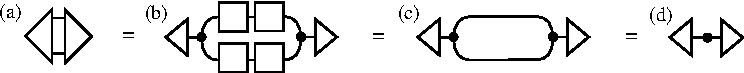
\includegraphics[width=14\xxxscale]{J1-norm}
\end{center}
The white boxes (valence-two tensors) represent unitary maps.  They therefore cancel 
resulting in the network illustrated in (c).  The \COPY-tensor
contracted as in (c) results in the identity wire (recall Figure (e) in Definition \ref{def:copy-prop}).  We then find the
inner product of the triangular tensors containing singular values,
\be 
\Rightarrow J_1 = \sum_i \lambda_i^2 = \lambda_0^2 +\lambda_1^2~ (= 1~\text{for a normalized state}) 
\ee 
Which is the desired result.  
\end{proof}
\end{lemma}



In addition to the norm $J_1$, for pure two-qubit states 
one finds another independent invariant given as\sn{A way to understand why we can expect only two invariants for two pure qubits is by considering the reduced density operator of a single qubit.  This can be done because there is only one possible partition for a two-qubit state.  This density operator has two singular values and we should be able to find (algebraically independent) invariants that separate the orbit, based on these two singular values. } 
\begin{equation}\label{eqn:J2} 
J_2 =  \sum \alpha^{i j}\alpha^{k l}\overline{\alpha}_{i l}\overline{\alpha}_{kj}
\end{equation} 
The invariant is at quartic order and its tensor diagram is given by contracting two copies of the state, and two copies of its dual under the dagger.
\begin{center}
 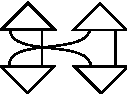
\includegraphics[width=2\xxxscale]{J2}
\end{center}

\begin{lemma}[Graphical contraction of $J_2$]
The graphical language enables a sequence of tensor contractions to relate the polynomial invariant $J_1$ to the singular values of the state.

\begin{proof}
From the graphical expression of $J_2$ (a) we arrive at (b) which is found from applying the diagrammatic SVD to (a).  
The two pairs of unitary order-two tensors cancel (c) and after contraction we are left with
a product of four valence-one triangles (d).  The center portion, attached to the four triangles (c) contracts to a single valence-four \COPY-tensor as\mn{This elementary property of contraction, can also be seen as the \textit{special} case of a more general normal form, see page 64 of \cite{FA}.  It can also be seen as a tensor version of node equivalence in digital circuits \cite{CTNS}.} 
\be 
\delta^i_{~jk} \delta^q_{~rs}\delta^{js}_{~~l}\delta^{rk}_{~~~m} = \delta^{iq}_{~~lm}
\ee 
$J_2$ thus becomes a product of singular values and hence (b) provides a
graphical variant of \eqref{eqn:J2} given as 
\be
J_2 = \sum_i \lambda_i^4 =  \lambda_0^4 + \lambda_1^4 = 1 - 2\lambda_1^2 + 2 \lambda_1^4
\ee 
where the last step follows from the constraint on the states norm.  
\begin{center}
 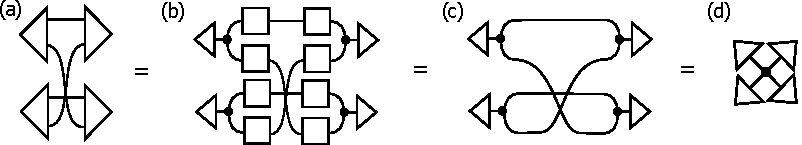
\includegraphics[width=14\xxxscale]{J2-explained1}
\end{center} 
\end{proof}
\end{lemma}



These graphical contractions inspired the following derivations.  

\begin{lemma}[General formulas equating state coefficients to singular values]
 Given a general two-qubit state
\begin{equation}
|\Psi\rangle = \alpha \ket{00} + \beta \ket{01} + \gamma \ket{10} + \delta \ket{11}
\end{equation} 
it can be shown that the Schmidt coefficients are given as 
\begin{equation}
\lambda_{1,2}^2=\frac{1}{2}\left( 1 \pm \sqrt{1-4|\beta\gamma - \alpha\delta|^2} \right)
\end{equation} 
where $\alpha$, $\beta$, $\gamma$, and $\delta$ are complex numbers.
\end{lemma}

\begin{corollary}
 The invariance of $J_2$ implies the invariance of the Schmidt coefficients and vise versa.
\end{corollary}
\begin{proof}
It can be shown that the invariant $J_2$ can be expressed as 
\begin{equation} 
J_2=1-2 |\beta\gamma - \alpha\delta|^2  
\end{equation} 
which implies that 
\be 
|\beta\gamma - \alpha\delta|^2=\frac{1-J_2}{2}
\ee 
and therefore
\begin{equation}
\lambda_{1,2}^2=\frac{1}{2}\left( 1 \pm \sqrt{2J_2-1} \right)
\end{equation}  
\end{proof}

\begin{remark}[Relating $J_2$ to entanglement]
 Parameterizing $\lambda_0:= \cos \theta$ and $\lambda_1:= \sin
\theta$, with $0\leq \theta \leq \pi/4$ (which gives $\lambda_0 \geq
\lambda_1$) the invariant $J_2$ becomes
\be 
J_2(\theta) = \cos^4 \theta + \sin^4 \theta= \frac{1}{4} (3 + \cos(4 \theta))
\ee 
where the last line again follows from the norm.  The angle $\theta$
now becomes a characterization of the entanglement.  $\theta = 0$ iff
the state is separable and $\theta = \pi /4$ iff the state is locally
equivalent to a maximally entangled Bell state.  We can see this from
the following plot of $J_2(\theta)$.  For small angles, the value of the plot is $\approx1$ as the angle increases, 
the entanglement increases and the value of $j_2$ goes to its maximum value of one half (at $\theta/\pi = 1/4$). 
%\yo{FIXME how?}
\begin{center}
 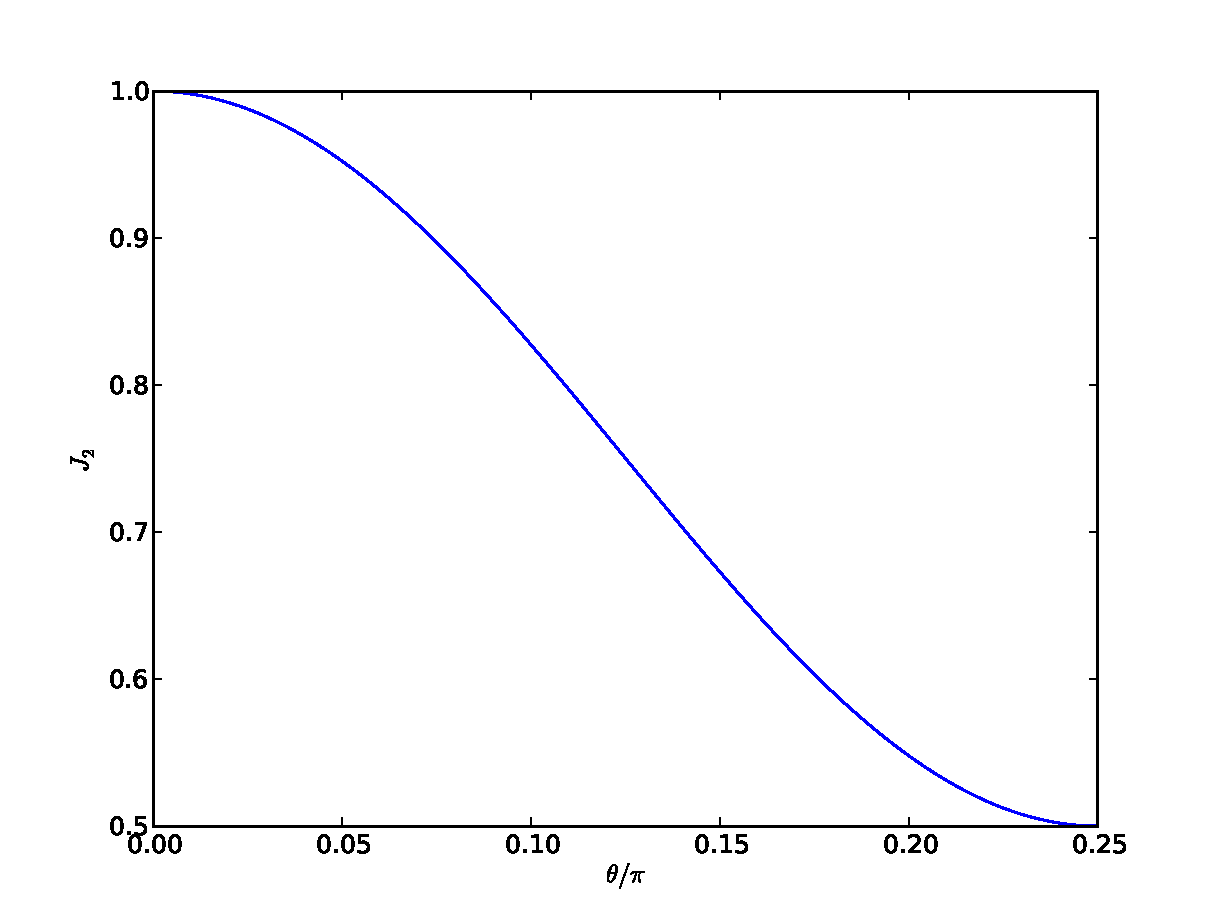
\includegraphics[width=0.65\textwidth]{J2_plot}
\end{center}
\end{remark}
% NOTE I can't read the labels, though the plot looks good, I can't actually see what is on the axis, at least 
% not on my small screen.  


\begin{remark}[Algebraic independence of $J_1$ and $J_2$: the fundamental ring]
$J_1$ and $J_2$ are the only algebraically independent invariants under local action of the unitary group.
Any polynomial function of such invariants is also a polynomial
invariant.  In this fashion, it is a remarkable feature that functions
of $J_1$ and $J_2$ are all that is needed to express any local unitary
invariant of two-qubit pure states.  This elementary result follows from a
much more powerful and general result in classical invariant theory.
That is a proof by Hilbert that the ring of polynomial invariants is
finitely generated \cite{hilbert}.  This corresponds to freely
generated linear sums and products of $J_1$, $J_2$ (the ring \begin{equation}
    \{J_1, J_2, (\R, +, \cdot)\}. 
\end{equation}
Any minimal complete set of invariants that
can freely generate the full ring are called \emph{fundamental invariants}.
\end{remark}

% \begin{remark}[Group orbits]
% \label{theorem:orbits}
% It is now well known (dating back to Hilbert) that the orbits of a compact linear group acting in a real vector space are
% separated by the (polynomial) invariants.
% %\yo{FIXME what's the content of this remark? Merge with the previous one?}
% \end{remark}

\paragraph{$n$-qubit LOCC invariants.}

The method we have described in detail for two qubits is readily extended to $n$-qubits.  
Consider the general expression for an $n$-qubit pure state 
\be 
\psi = \sum \psi_{ijk...}\ket{ijk...}
\ee 
A general polynomial of the state coefficients together with their complex conjugates is expressed as
\begin{equation}\label{eqn:n-qubit-invariant}
\sum c^{ijk...}_{qrs...lmn}\overline{\psi}^{qrs...}\overline{\psi}^{lmn...}\cdots\psi_{ijk...}\cdots
\end{equation} 

If the polynomial \eqref{eqn:n-qubit-invariant} has an equal numbers of $\psi$’s 
and $\overline{\psi}$’s and all the indices of the $\psi$ are contracted using the
invariant tensor $\delta$ with those of the $\overline{\psi}$, each index being
contracted with an index corresponding to the same party then the polynomial is 
manifestly invariant under LOCC transformations.

\begin{remark}[Connection to the diagrammatic language] 
Invariant polynomials \eqref{eqn:n-qubit-invariant} can be written in terms of permutations
on the indices, and given diagrammatically as contraction with a permutation operator.  
\end{remark}

\begin{remark}[Fundamental ring of invariants]
Although we can generate a full basis of invariants \eqref{eqn:n-qubit-invariant}, except in rare cases, a minimal set of invariants is not known. 
\end{remark} 

\subsubsection*{Tensor contraction for SLOCC\sn{SLOCC: Stochastic Local Operations and Classical Communication.} invariants}   
SLOCC equivalence amounts to equivalence under local invertible 
transformations. This results in a coarser partitioning of the set of states 
as compared to LOCC equivalence, since SLOCC shows which states are
accessible to different parties with non-zero probability.  The following result was proven in \cite{3qubits}.  

\begin{theorem}[SLOCC]\label{theorem:SLOCC}
Two states are SLOCC-equivalent iff there exists
an invertible local operator relating them given by the action of the local general linear group \cite{3qubits} 
\be 
GL(d_1, \C)\times GL(d_2, \C)\times \ldots  \times GL(d_n, \C). 
\ee 
\end{theorem}

\begin{remark}[SLOCC under the special linear group]\label{remark:SL}
Up to a scale factor, and without loss of generality, we will instead consider action of the special linear group, $SL(2,\C)$ on qubits.  
\be
SL(2, \C) \times SL(2, \C) \times \ldots  \times SL(2, \C) 
\ee 
The precise relation between $GL$ and $SL$ invariants is mentioned in Remark \ref{remark:GL-vs-SL}.  We then consider transforming an $n$-party state $\psi$ to $S\ket{\psi}$ with $S:= \bigotimes_{i=0}^n S_i$ where each $S_i$ has unit determinant.  Action of either group is known to correspond precisely to quantum operations that preserve true entanglement under a general quantum operation.  
 
\end{remark}
 


\paragraph*{Graphical properties of the Levi-Civita symbol.} In order to study 
SLOCC invariants, and their tensor networks, we will need to recall 
the Levi-Civita symbol and consider a tensor network representation.  

\begin{definition}[Levi-Civita symbol]
The order-$n$ Levi-Civita symbol $\varepsilon^{ij \cdots k}$
is the fully antisymmetric tensor with coefficients in $\{-1,0,1\}$.
All its legs have the same dimension $d = n$.
\be
\varepsilon^{ij \cdots k} = \left\{
\begin{array}{rl}
1  & \text{when} \: (i,j,\ldots, k) \: \text{is an even permutation of the index values,}\\
-1 & \text{when} \: (i,j,\ldots, k) \: \text{is an odd permutation, and}\\
0  & \text{otherwise}.
\end{array}
\right.
\ee

% Diagrammatically it is represented as

% \yo{FIXME finish}

% TODO we need to be careful with terminology here, the Levi-Civita
% symbol is _not_ a tensor in the diff.geom. sense. What about here?

% ah, well let's think about this but everything that is a linear map is a tensor in our setting here.  
% we should explain this point here.  
\end{definition}

Before proceeding to an analysis of the SLOCC invariant tensor network structure, we must explore some properties of the epsilon tensor.  

\begin{remark}[Matrix determinant]
The determinant for an $n$-by-$n$ matrix
$A$ can be expressed in terms of the Levi-Civita symbol as follows:
\be
\label{eq:epsilon-det}
\det (A) = \varepsilon^{i_0 \cdots i_{n-1}} A\indices{^{0}_{i_0}} \cdots A\indices{^{n-1}_{i_{n-1}}}.
\ee
Diagrammatically,
the determinant takes the form
\begin{center}
 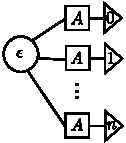
\includegraphics[width=2.5\xxxscale]{det}
\end{center}
or equivalently, the determinant is directly proportional to the expected value of the operator 
\begin{equation}
   \bra{\epsilon} \bigotimes_{i=1}^n A_i \ket{\epsilon} 
\end{equation}
with respect to the epsilon state in that dimension $n$. 
\end{remark}


\begin{lemma}[Invariance of epsilon under $SL(n, \C)$]
\label{lemma:epsilon-invariance}
We will consider the representation $L$ of the group $SL(n, \C)$ on
${\C^n}^{\otimes n}$, defined as
\be
L(S) \ket{\psi} := S^{\otimes n} \ket{\psi},
\ee
where $S \in SL(n, \C)$.
The order-$n$ epsilon state is invariant under this representation:
\begin{align*}
L(S) \ket{\varepsilon}
&= S\indices{^{i'}_i} S\indices{^{j'}_j} \cdots S\indices{^{k'}_k}
\varepsilon^{ij\cdots k} \ket{i' j' \cdots k'}
= \varepsilon^{i'j' \cdots k'} \ket{i' j' \cdots k'} = \ket{\varepsilon}.
\end{align*}
\end{lemma}

\begin{proof}
If an index value is repeated in the set~$\{i', j', \ldots, k'\}$,
the antisymmetry of epsilon dictates that the expression must
vanish. Hence the only nonvanishing index combinations are
permutations of the $n$ allowed index values.
Using~\eqref{eq:epsilon-det}, we can see that the permutation
$$
(i', j', \ldots, k') = (0, 1, \ldots, n-1)
$$
corresponds to
$\det(S)$, which equals~$1$ since $S \in SL(n, \C)$.
Invoking the antisymmetry of epsilon again we conclude that all even
permutations must also yield~$1$, and all odd permutations~$-1$, thus
recovering the definition of epsilon.

%In fact, $\psi_\varepsilon$ carries the trivial representation of $S\otimes S$ (this is actually a special case of Schur-Weyl Duality).  So 
%$S\otimes S\psi_\varepsilon = \psi_\varepsilon$ which results in the diagrammatic equation 
\begin{center}
 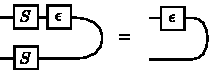
\includegraphics[width=4\xxxscale]{epsilon-invariants1}
\end{center}

%as can be checked by considering the general form of an $SU(2)$ matrix as 
%\be
%S = \alpha \ket{0}\bra{0} + \overline{\alpha}\ket{1}\bra{1} + \beta \ket{1}\bra{0} - \overline{\beta}\ket{0}\bra{1}.
%\ee 
However, we will then note that under wire duality we arrive at the relation 
\begin{center}
 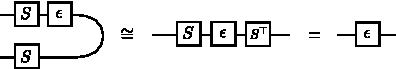
\includegraphics[width=8\xxxscale]{epsilon-invariants-II}
\end{center} 
which says that $S\varepsilon S^\top = \varepsilon$.   So under wire duality, we find that $(S\otimes S) \psi_\varepsilon \cong S\varepsilon S^\top$.  
\end{proof}


% 1. The determinant of an n\times n matrix A = (aij) can be written as
% 
%         \det A = \varepsilon_{i_1\cdots i_n} a_{1i_1} \cdots a_{ni_n},
% 
% where each il should be summed over 1,\ldots, n.
% 
% Equivalently, it may be written as
% 
%         \det A = \frac{1}{n!} \varepsilon_{i_1\cdots i_n} \varepsilon_{j_1\cdots j_n} a_{i_1 j_1} \cdots a_{i_n j_n},
% 
% where now each il and each jl should be summed over 1,\ldots, n.

\begin{remark}[Defining equations relating $\delta$ and $\epsilon$]
 It is a classical result of invariant theory that every identical relation satisfied by contractions of $\delta$'s and $\epsilon$'s can be built up from the following relations (see e.g.\ \cite{Penrose67}).  
 \be 
 \epsilon_{AB}=-\epsilon_{BA}; ~~~~~~~~~~ \epsilon^{AB} = -\epsilon^{BA}
 \ee
 \be 
 \delta^B_A\delta^C_B=\delta^C_A; ~~~~~~~~~ \delta^B_A\epsilon^{AC}; ~~~~~~~~ \delta^B_A\epsilon^{AC}=\epsilon^{BC}; ~~~~~~~~ \epsilon_{AB}\epsilon^{AC} = \delta^C_B
 \ee
 \be 
 \delta^A_A = 2 = \epsilon_{AB}\epsilon^{AB}
 \ee 
 Also, the identity, 
 \be 
 \epsilon_{AB}\epsilon_{CD} + \epsilon_{AD}\epsilon_{BC} + \epsilon_{AC}\epsilon_{DB} = 0
 \ee 
 holds, together with the equivalent identities obtained by raising indices of the above, with Levi-Civita symbols, e.g. 
 \be 
 \delta^B_A\delta^D_C - \delta^D_A\delta^B_C= \epsilon_{AC}\epsilon^{BD}
 \ee  
 We also note that when we assign values to $A, B=0,1$ we arrive at the following relations, between the indices and the tensor components as 
 \be 
 \epsilon_{AB}= A-B
 \ee 
 \be 
 \delta^A_B = 1 - (A-B)^2 
 \ee 
\end{remark}

\begin{remark}[Matrix determinant in dim $=2$]
The case of the determinant in two dimensions becomes
\be 
\sum \varepsilon_{ij}A_{i0}A_{j1} = \varepsilon_{01}A_{00}A_{11} +  \varepsilon_{10}A_{10}A_{01}
\ee 
where $\varepsilon_{10} = -1$ and $\varepsilon_{01} = 1$.  
In two dimensions, when all $i,j,m,n$ are in $\{0,1\}$, the following identities hold.  
\be 
\varepsilon_{ij} \varepsilon^{mn} = \delta^m_i \delta^n_j - \delta^n_i \delta^m_j
\ee 
\be 
\varepsilon_{ij} \varepsilon^{in} = \delta^n_j
\ee 
\be 
\varepsilon_{ij} \varepsilon^{ij} = 2
\ee   
\end{remark}

\begin{remark}[Epsilon symbol in two dimensions]
In two dimensions the Levi-Civita symbol is an element of the Pauli group:
$\varepsilon = i Y = -XZ = ZX$, that is,\footnote{Note that the diagram is not written using the convention 
from quantum circuits, where the order of composition of operations in an equation is reversed in the circuit.} 
%\yo{FIXME diagram is wrong}
\begin{center}
 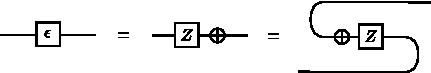
\includegraphics[width=8\xxxscale]{epsilon-tensors}
\end{center}
where the last step of bending output to inputs and inputs to outputs
takes the transpose of a linear map.
%The order-two tensor $\varepsilon$ is in the Pauli group which is a
%subgroup of the Clifford group of quantum circuits, any dynamics of
%which are known to be efficient to simulate on a classical computer.
% \psi_\varepsilon := \ket{01}-\ket{10}
\end{remark}

\paragraph*{SLOCC invariants.}
For pure two-qubit states, the single $SL$ invariant is the determinant
of the coefficient matrix $\alpha$ as 
%\yo{FIXME proof}
\begin{equation}\label{eqn:K1}
K_1 = \sum \varepsilon_{i j}\varepsilon_{k l} \alpha^{i k} \alpha^{j l}  = 2\det (\psi^i_{~j}) = 2(\alpha^{00}\alpha^{11} - \alpha^{01}\alpha^{10})
\end{equation}
here $\varepsilon$ is the fully antisymmetric tensor on two indices defined as $\varepsilon_{00} = \varepsilon_{11} = 0$ and $\varepsilon_{01} = -\varepsilon_{10}$.  

\begin{remark}
 The norm is not a SLOCC invariant.  
\end{remark}

\begin{remark}[Algebraic independence of $K_1$: the fundamental ring]
 Any other polynomial invariant of the induced action of the special linear group is necessarily a polynomial in $K_1$. Since there is only one invariant in this special case, each member of this class could be considered a fundamental invariant.  Finding the fundamental invariants becomes complicated for higher dimensional systems.  
\end{remark}

With the epsilon identities in place, we are now able to consider the tensor structure of~$K_1$:
\begin{equation}\label{eqn:K_1} 
K_1 = \sum \varepsilon_{i j}\varepsilon_{k l} \alpha^{i k} \alpha^{j l} 
\end{equation}


\begin{lemma}[Diagrammatic contraction of $K_1$]
 The diagrammatic language contracts the tensor network for $K_1$ \eqref{eqn:K_1} to be twice the determinate of the matrix of state coefficients $(\bra{\Phi^+}\otimes \I)\ket{\psi}$ found from bending a wire on $\psi$. 
 \end{lemma}
 
 \begin{fullpage}
 \begin{proof}[Diagrammatic contraction of $K_1$]
In the following figure, (a) represents $K_1$ which simplifies to (d) using our previous results.  
\begin{center}
 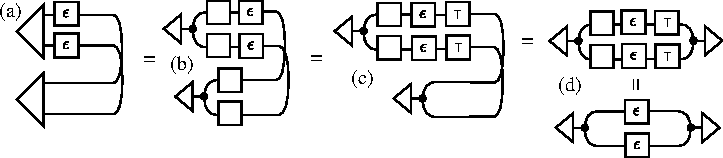
\includegraphics[width=15\xxxscale]{K1}
\end{center} 
In (c) we have added $\top$ symbols in the unitary boxes, to denote transpose as found from sliding a box around a bent wire.  Figure (d) shows the $SU(2,\C)$ invariant of $\varepsilon$ as in Lemma \ref{lemma:epsilon-invariance}.   

To continue the analysis of this network, we will need to introduce a few more identities that we have proven in detail elsewhere \cite{CTNS, BB11}.  We need to then consider the stabilizer group of the \COPY-tensor.  This is an eight element group 
\be 
\{\I, X\otimes X\otimes X, -X\otimes Y\otimes Y, -Y\otimes X\otimes Y, -Y\otimes Y\otimes X, Z\otimes Z\otimes \I, Z\otimes \I\otimes  Z, \I\otimes  Z\otimes Z\}
\ee 
and then we consider the diagrammatic laws on a choice of generators 
\begin{center}
 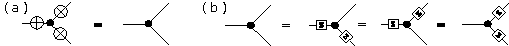
\includegraphics[width=17\xxxscale]{copy-stabs}
\end{center} 
From these identities we then return to our equation for the determinant.  
\begin{center}
 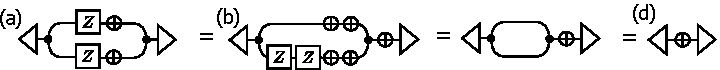
\includegraphics[width=16\xxxscale]{K1-final1}
\end{center} 
In (a) we express epsilon in using the Pauli algebra.  In (b) we apply the fact that the \COPY-tensor is stabilized
by the tensor product of three bit flip operators $X\otimes X\otimes
X$, as well as pair products of $Z$'s.  We combine this with the
fact that $X^2=\I = Z^2$ to show that the internal order-two tensors
all cancel out in (b).  This results in the network (d).  What remains
is one bit flip operator.  It can be contracted with an valence-one
triangular tensor, performing the map $\lambda_i \mapsto \lambda_j$
for $i\neq j$.  This leads to the inner product
\be 
(\lambda_0, \lambda_1).(\lambda_1, \lambda_0) = 2\lambda_1\lambda_0 = 2\det (\psi) 
\ee 
which matches precisely what we expect.  
\end{proof}
\end{fullpage}
 

 In Theorem \ref{theorem:SLOCC} we recalled the definition of SLOCC invariance, with respect to $GL$, the general linear group.  We then stated that there is a connection to the special linear group in Remark \ref{remark:SL}.  We make this connection precise in the following remark.  
 
\begin{remark}[Relating GL and SL in SLOCC]\label{remark:GL-vs-SL}
Let $G\in GL$.  We have that $\det(G)= k$, for some constant $k$ and
that $S\in SL$ has $\det(S)=1$.  Let $S = w G$, then letting 
\be 
w = \frac{1}{\det(G)^{\frac{1}{n}}}, ~ \Rightarrow ~ \det(S)=\det{wG}=1
\ee 
From this it follows that 
\be 
G \ket{\psi} = \det(G)^{\frac{1}{n}}S\ket{\psi}
\ee 
and so the transformations are related by constant factors (global scale factor).  Each polynomial SLOCC invariant is a homogeneous function with respect to this global scale factor.  The invariant changes only by a factor that does not depend on the state, but only on the transformation $G,S$.  
\end{remark}

\begin{fullpage}
\begin{example}[Calculated Values of the Invariants for Example States]
Here we calculate the values of each invariant for several common states of interest. The reduced \AND-state is found from recalling Equation \eqref{eqn:AND-map}.  
\begin{equation}
 \wedge_{ij}^{~~k}=(\ket{00}+\ket{01}+\ket{10})\bra{0} + \ket{11}\bra{1}
\end{equation}
We evaluate this Boolean tensor at $k=0$ as 
\begin{equation}
 \wedge_{ij}^{~~0}=\left(\ket{00}+\ket{01}+\ket{10})\bra{0} + \ket{11}\bra{1}\right)\ket{0} = \ket{00}+\ket{01}+\ket{10}
\end{equation}

\begin{center}
\begin{tabular}{r||c|c|c|c}
Type & State & $J_2$ & $K_1$ & $(\lambda_0, \lambda_1)$ \\\hline \hline
Product  & $\ket{0}\ket{0}$ & 1  & 0 & $(1,0)$\\\hline
Bell  & $\frac{1}{\sqrt 2}(\ket{00}+\ket{11})$ & $\frac{1}{4}$ & $\frac{1}{2}$ & $\frac{1}{\sqrt 2}(1,1)$ \\\hline
 \AND-type & $\frac{1}{\sqrt 3}(\ket{01}+\ket{10}+\ket{00})$  & $\frac{7}{9}$ & $\frac{1}{3}$ & $\lambda_\pm=\sqrt{\frac{1}{6} \left(3\pm\sqrt{5}\right)}$\\\hline 
General & $\sqrt{\lambda}\ket{00}+\sqrt{1-\lambda}\ket{11}$ & $2\lambda(\lambda-1)+1$ & $2\sqrt{\lambda(1-\lambda)} $ & $(\sqrt{\lambda}, \sqrt{1-\lambda})$ 
\end{tabular}
\end{center}
\end{example}
\end{fullpage}


\subsection*{Invariant composition law} 

Consider two initially non-interacting quantum wavefunctions $\ket{\psi}$ and $\ket{\phi}$.  If these states interact by a coupling unitary propagator $U$, the polynomial invariants of each state individually are not necessarily polynomial invariants, of the join system $U\ket{\phi}\otimes\ket{\psi}$.  

It is desirable to devise methods to compose invariants.  By this we mean that if we know the polynomial invariants of $\ket{\psi}$, $\ket{\phi}$ and $U$, together with a tensor network defining their composition, from this information alone, how can we determine the resulting invariants of the joint system?  In the present section, we solve this problem for the case of bipartite systems of equal dimension.  

\paragraph{Composition of the invariant $K_1$}
We will consider a quantum state $\psi\in \7H\otimes \7H$.  We will act on this state locally on each leg, with invertible linear maps.  A possible scenario is depicted as follows.  On the left, we have a state $\in \7H\otimes \7H$ factored using the diagrammatic SVD.  
We then act on this state with invertible maps $S_1$ and $S_2$.  
\begin{center}
 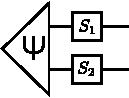
\includegraphics[width=2.5\xxxscale]{det-composition-I}
\end{center}

The invariant $K_1$ is equal to twice the determinate of the coefficient matrix, found from bending either wire back, on the tensor representing the state.  The invariant $K_1$ is equal to zero iff $\det(\psi)=0$.  This is true iff $\psi$ is separable, thereby partitioning the SLOCC class into a disjoint union: entangled vs. not. We can calculate $K_1$ for not only the state, but also for the maps $S_1$ and $S_2$.  Given the quantities 
\be 
K_1(\psi),~K_1(S_1), ~ K_1(S_2)
\ee 
we can deduce from the standard properties of the determinant, the value of the invariant found from acting on $\psi$ with the map $S_1\otimes S_2$ as 
\be 
K_1(S_1\otimes S_2 \psi)= K_1(\psi)K_1(S_1)K_1(S_2)
\ee
Such a scenario extends to the case of qudits, and the value of the invariants evaluates to the product of singular values of all parties in the contracted network.  

%Composition of the invariant $J_2$ is considered in \cite{BBL11}.  


% \yo{Need to double check this subsection.} The situation is more subtle in the case of $J_2$. Assume two 2-qubit quantum states with invariants:
% \begin{eqnarray}
% J_a &=& \alpha^{ij}~\alpha^{kl}~\bar\alpha_{il}~\bar\alpha_{kj} \\\nonumber
% J_b &=& \beta^{ij}~\beta^{kl}~\bar\beta_{il}~\bar\beta_{kj}
% \end{eqnarray} 
% If both states are composed together, then they will have the invariant:
% \begin{equation}
% J_c = \gamma^{ij}~\gamma^{kl}~\bar\gamma_{il}~\bar\gamma_{kj}
% \end{equation} 
% where:
% \begin{equation}
% \gamma^{ij}=\alpha^{il}~\beta^{lj}
% \end{equation} 
% 
% Then:
% \begin{eqnarray}
% J_c &=& \gamma^{ij}~\gamma^{kl}~\bar\gamma_{il}~\bar\gamma_{kj}  \\\nonumber
% &=& \alpha^{im}~\beta^{mj}~~\alpha^{kn}~\beta^{nl}~~\bar\alpha_{ip}~\bar\beta_{pl}~~\bar\alpha_{kq}~\bar\beta_{qj} \\\nonumber
% &=& \alpha^{im}~\alpha^{kn}~\bar\alpha_{ip}~\bar\alpha_{kq}~~~\beta^{mj}~\beta^{nl}~\bar\beta_{pl}~\bar\beta_{qj} \\\nonumber
% &=& U^{mn}_{pq}~V^{mn}_{pq}
% \end{eqnarray} 
% where:
% \begin{eqnarray}
% U^{mn}_{pq}&=& \alpha^{im}~\alpha^{kn}~\bar\alpha_{ip}~\bar\alpha_{kq} \\\nonumber
% V^{mn}_{pq} &=& \beta^{mj}~\beta^{nl}~\bar\beta_{pl}~\bar\beta_{qj}
% \end{eqnarray} 
% 
% If we require that 
% \begin{equation}
% J_c\propto J_a
% \end{equation} 
% then $V^{mn}_{pq}$ needs to satisfy:
% \begin{equation}
% V^{mn}_{pq}\propto \delta^m_q~\delta^n_p
% \end{equation} 
% which means that:
% \begin{eqnarray}
% \beta^{mj}~\bar\beta_{qj}&\propto& \delta^m_q \\\nonumber
% \beta^{nl}~\bar\beta_{pl}&\propto& \delta^n_p
% \end{eqnarray} 
% and it is satisfied by states of the form:
% \begin{equation} 
% |\psi\rangle_b = \alpha |00\rangle + \beta |01\rangle \pm \beta |10\rangle \mp \alpha |11\rangle
% \end{equation} 
% with an invariant:
% \begin{equation}
% J_b=\frac{1}{2}
% \end{equation} 
% which corresponds to a maximally entangled state.




\section{Generating Invariants for General Density Operators}
A method to systematically generate polynomial invariants of density
operators acted on by the local unitary group exists and was shown to
me by Markus Grassl \cite{entinv2}.  Here we will cast this method into the Penrose tensor calculus.  The method generates a complete basis of monomials that are necessarily
invariants of the local unitary group acting on a density matrix.  A polynomial invariant 
could be expressed in this complete basis.  Although we can generate a complete basis of invariants, except in rare cases, finding the minimal collection of polynomial invariants is computationally difficult.  A utility of generating this basis, comes from the fact that the tensor networks we consider can be used to calculate any properties that are invariant under the action of the local unitary group.  This includes R\'{e}nyi entropies and the entanglement spectrum.  

\paragraph{The invariant basis.}  Consider a density 
operator $\rho\in \7H\rightarrow \7H$.  We can write 
this in a basis and consider acting on $\rho$ by a given a group $G$.  
A polynomial in 
\be 
f(x_0, x_1, x_2, x_3, \overline{x}_0, \overline{x}_1, \overline{x}_2, \overline{x}_3)=:f(\1x) 
\ee 
is invariant under $G$ iff $\forall g\in G$ 
\be 
f^g(\textbf x) = f(\textbf x) 
\ee 
where the notation $f^g(\textbf x)$ means 
% \yo{FIXME explain what T and multiplication by g means i.e. define the action}
% @Ville: can you do this? 
\be 
f\small{\left(\left[g(\textbf x)^\top \right]^\top\right)} = f\left[(\textbf x)g^\top \right]
\ee 
so we let $g$ act on $\textbf x$ and then let $f$ act --- $f$ is constant under $G$ iff $f$ is invariant.  

The question we are considering is how to generate 
a complete monomial basis where each basis element is invariant under $G$.  This would then imply that any holomorphic function, can be written in this basis.  In fact, such a function would (i) necessarily be invariant under $G$ and (ii) be a function of the density operator $\rho$.    

%\yo{FIXME why a monomial basis? isn't the idea to *expand* invariants in a
%monomial basis, but the basis elements themselves need not be invariant?}
% @ Ville: I changed and improved this, what do you think now? 
% yeah, but finding a minimal set is hard, @ Ville: what do you think now?   

First consider the network 
\begin{center}
 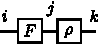
\includegraphics[width=2.5\xxxscale]{generating-invariants}
\end{center}
representing the equation $F^i_{~j}\rho^j_{~k}$ then Tr$(F\rho)=\delta_{ik}F^i_{~j}\rho^j_{~k}$ that is 
\begin{center}
 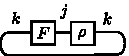
\includegraphics[width=4\xxxscale]{generating-invariants-trace1}
\end{center}
$= F^i_{~j}\rho^j_{~i}$ If we were considering 
\be 
\rho = x_0\ket{0}\bra{0} + x_1\ket{0}\bra{1} + x_2 \ket{1}\bra{0} + x_3 \ket{1}\bra{1}
\ee 
then this trace would evaluate to 
\be 
F_{00}x_0 +F_{01}x_1 + F_{10}x_2 + F_{11}x_3
\ee 
and we can pick an valence-four $F$ such to expand the second order monomials as Tr$(F\rho^{\otimes 2}) = F^{il}_{jk}\rho^j_i\rho^l_k$ which translates to the tensor network as 
\begin{center}
 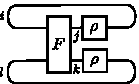
\includegraphics[width=4\xxxscale]{monomial-21}
\end{center}
This procedure carries on in this fashion, arriving at a monomial of order $n$ as 
\be 
\Tr(F\rho^{\otimes n}) = F^{il\cdots q}_{jk\cdots r}\rho^j_i\rho^l_k\cdots \rho^q_r
\ee 
The question then changes.  We have generated a complete basis in the coefficients of the density operator, with coefficients in $F^{il\cdots q}_{jk\cdots r}$.  We then will act on 
the density operators by elements $g\in G$ 
\be 
\rho' = g \rho g^{-1}
\ee 
and search for $F^{il\cdots q}_{jk\cdots r}$ that satisfy 
\begin{equation}\label{eqn:density-invariant} 
\Tr(F g^{\otimes n} \rho^{\otimes n}g^{\otimes n -1}) = \Tr(F \rho^{\otimes n})
\end{equation}  
Equation \eqref{eqn:density-invariant} is satisfied by monomial invariants.  From this it follows that 
\begin{equation} 
\Tr(F g^{\otimes n} \rho^{\otimes n}g^{-1\otimes n }) = \Tr(\rho^{-1\otimes n }F g^{\otimes n} g^{\otimes n})
\end{equation}  
$\forall \rho$ and so 
\be 
[F, g^{\otimes n}]=0, ~\forall g\in G
\ee 
We are then faced with finding matrices $F$ that commute with $g^{\otimes n}$ for each $g\in G$. This problem was solved in a different setting around 1937, and the solution is roughly stated in the following theorem.  

\begin{theorem}[R. Brauer, 1937]
 The algebra of matrices that commute with each $U^{\otimes n}$ for $U \in  U(n)$ is
generated by a certain representation of the permutation group.
\end{theorem}

The permutation group has a well known and evident diagrammatic form. In (a) we show the elements of the permutation group on one system.  In (b) we show the elements on two systems.  (c) Illustrates the permutation group on three elements, $S_3$ of order $6$.\sn{Of possible related interest, is the diagrammatic presentation of the Temperly-Lieb algebra \cite{TL07}.} 
\begin{center}
 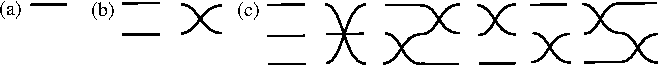
\includegraphics[width=14\xxxscale]{symmetric-group}
\end{center}
We then carry on to evaluate 
\be 
\Tr(S_k g^{\otimes n} \rho^{\otimes n}\rho^{-1\otimes n})
\ee 
to form invariant monomials.  We consider the case where we wish to generate an order one invariant 
in (a) below.  Order two invariants are found below in (b).  We note that the first invariant is simply the square of the invariant 
found in (a).  The second however, is independent.  An example of an invariant of order three is given in (c). The situation continues.  The basis is finitely generated form the Cayley-Hamilton Theorem.  We have that every density operator satisfies its own characteristic polynomial, giving an $n$th order polynomial equation in $\rho$ that vanishes.  
\begin{center}
 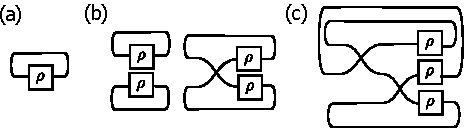
\includegraphics[width=10\xxxscale]{trace-symmetric-invariants1}
\end{center}

%\yo{TODO note that each subsystem in the state gets its own $S_k$ permutation independently of the others.}  @ ville: what are you talking about?  Sorry, don't understand.  
\paragraph{The general form.}  We consider the monomial invariant generated by tracing over the contraction with the SWAP-operator in (a) below.  Here we have acted on $\rho$ with some unitary operation $U$, and give a diagrammatic proof that the network contracts to a quantity that is invariant, under unitary transformations of $\rho$.  

To see this, we slide $U, U^\dagger$ around the bends, resulting in (b).  The diagram reduces to (c), showing that the invariant evaluates to $\Tr(\rho^2)$.  
\begin{center}
 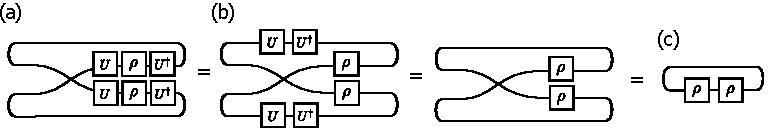
\includegraphics[width=14\xxxscale]{trace-symmetric-invariants-example1}
\end{center}

\begin{remark}[Generating a complete basis of invariants by tensor contraction]
To generate a complete basis, we have to consider operations like SWAP that permute all elements to different elements. These are called complete permutations.   
\end{remark}

\begin{lemma}[Diagrammatic proof of the basis]
 Every complete permutation on $n$ wires contracted with $n$ tensor copies of $\rho$ and traced over, contracts to the elementary diagram giving the trace of $\rho^n$.  
\end{lemma}

The unitary invariants of any contraction with a complete permutation operator is readily shown diagrammatically.  Any complete permutation is can be shown to contract to (a) below.  It then possible to understand a complete basis of invariants by evaluating the quantity  as shown in (c) below.  
\begin{center}
 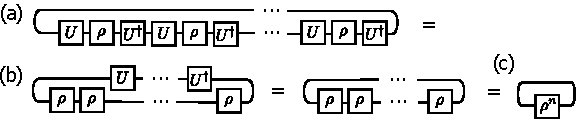
\includegraphics[width=14\xxxscale]{trace-n1}
\end{center}
Note that in (b), we have pulled both of the unitaries around bends.  We should have written $U^\top$ and $U^{\dagger\top}$ but we have omitted the transpose symbol $\top$ for ease of producing the figures.  These unitary maps still contract to identity as is quickly verified.  




\begin{example}[Trace invariants for qubit density operators]
We will consider generating the fundamental invariants for a qubit density operator.  
The first invariant follows from tracing over the identity operator (the only permutation group element on a single system) 
\be
I_1 =\Tr(\rho)
\ee 
is the constant norm.  The second is 
\be
I_2 = \Tr(\rho^2)
\ee
which turns out to be precisely what is known in other areas of the literature as the purity.  In terms of the singular values we have 
\be
I_1=\lambda^+ + \lambda^- = 1
\ee
which is the norm and 
\be
I_2=\lambda_+^2 + \lambda_-^2 
\ee
For the purpose of generating polynomial invariants, it is enough to stop with $I_1$ and $I_2$.  In fact, from the Cayley-Hamilton Theorem, we have that there is a polynomial in second order in $\rho$, that vanishes identically.  In other words, constants $a,b,c$ exist such that 
\be 
a \rho^2 + b\rho + c \I = 0 
\ee 
so higher powers of $\rho$ can be expressed in terms of $I_1$ and $I_2$ through this relation.  These invariants are indeed algebraically independent and complete, meaning any other polynomial invariant can be expressed in $\{\R, +, \cdot, I_1, I_2\}$.  For instance, 
\be
\text{Det}(\rho) = \frac{1}{2}\left(\Tr(\rho)^2 - \Tr(\rho^2) \right)= \frac{1}{2}\left(I_1 - I_2\right)= 1 - (c^2+a^2+b^2)= \lambda_0\lambda_1
\ee
\end{example}


\subsection*{Topological equivalence of pure and mixed state invariants}

% the topology of the slocc and locc invariants for both pure and mixed states become totally 
% equvlient in the diam language 

We have considered pure state invariants as well as mixed state invariants, under 
the action of the local unitary group.  We will consider the relation between these two approaches, when cast into our diagrammatic framework.  \marginnote{{\it ``Any effect, constant, theorem or equation named after Professor X was first discovered by Professor Y, for some value of Y not equal to X.''} ---
John C.~Baez}

Let us return to the expression for $J_2$ 
\be 
J_2 = \sum \alpha^{i j}\alpha^{k l}\overline{\alpha}_{i l}\overline{\alpha}_{kj}
\ee 
We will then write 
\begin{equation}\label{eqn:J2-vs-B} 
\alpha^{i j}\overline{\alpha}_{il} =: B^j_{~l}
\end{equation} 
which is given graphically below.  
\begin{center}
 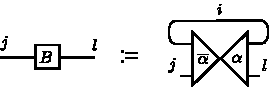
\includegraphics[width=6\xxxscale]{J2-rehashed-11}
\end{center} 
We also fix $B^l_{~j} := \alpha^{k l}\overline{\alpha}_{k j}$.  It now follows that 
the expression for $J_2$ becomes 
\be 
J_2 = \sum  B^l_{~j}B^j_{~l} = \Tr(B^2) 
\ee 
In (b) we see that this is found graphically when acting on two reduced states with a SWAP operation, and then tracing over the result.  
\begin{center}
 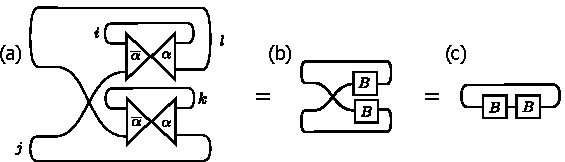
\includegraphics[width=12\xxxscale]{J2-rehashed1}
\end{center} 


We will go on to show that this invariant is in fact identical to the pure state invariant.  
From application of the graphical identity (Penrose's graphical representation of a density state is on the right) 
\begin{center}
 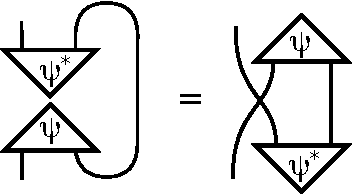
\includegraphics[width=4\xxxscale]{penrose-density-state}
\end{center} 
it now follows by applying this identity to (a) we arrive at the expression for $J_2$ we considered in Section \ref{sec:qubit-invariants}.  
\begin{center}
 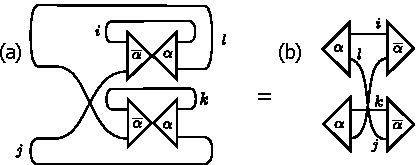
\includegraphics[width=10\xxxscale]{J2-mixed-vs-pure1}
\end{center} 


\section{Some Symmetries of \texorpdfstring{$\rho$}{}} 
We have expressed two Theorems (\ref{theorem:injection} and \ref{theorem:symmetry-class}) which relate density operators to quantum states precisely.  This might be thought of as a type of symmetry.  The other type of symmetry we have considered are invariant polynomials in the coefficients of a density operator.  These symmetries are general, as they are found for arbitrary density operators.    In the present section, we will remind the reader of other types of symmetry that are sometimes considered in quantum theory.  Symmetry plays a key role in the lectures that follow, so here is just an introduction.  In particular, symmetry will be considered in detail in Lecture III.  To begin, let us recall the typical symmetry that is often considered in quantum physics.  

\begin{example}[Group Symmetry of $\rho$]
 We will consider a general density operator $\rho$ and look for $V\in U(d)$ such that 
 \be 
 \rho = V\rho V^\dagger
 \ee 
 this implies that $[\rho, V]=0$ and we arrive at a basis for $G$ by noting the unitary operators that commute with $\rho$.  
 That is, $\{\ket{\lambda_i}\}_i$ such that $\rho = \sum_i p_i\ket{\lambda_i}\bra{\lambda_i}$.  It then follows from $VV^\dagger = \I$ that 
 every $V\in G$ can be written as 
 \be 
 V= \sum_i e^{i\theta_i}\ket{\lambda_i}\bra{\lambda_i}
 \ee 
\end{example}

In quantum computer science another symmetry is often considered.  This is the symmetry found by so called, \emph{stabilizer states}.  
We will discuss this in detail in Lecture III and also cover a bit of it in Lecture IV.  A quantum gate~$U$ which is a tensor product of Pauli operators is said to stabilize the state~$\ket{\psi}$ iff $U \ket{\psi} =
\ket{\psi}$. All the gates stabilizing a given state form a group.  

\begin{example}[Pauli stabilizers]
Here are some standard examples of states stabilized by the Pauli-group
\begin{itemize}\addtolength{\itemsep}{-0.25\baselineskip}
 \item[(i)] \textbf{Pauli-X}: $\sigma^x$ stabilizes $\ket{+}=\ket{0}+\ket{1}$
and $-\sigma^x$ stabilizes $\ket{-}=\ket{0}-\ket{1}$
 \item[(ii)] \textbf{Pauli-Y}: $\sigma^y$ stabilizes
$\ket{y_+}=\ket{0}+i\ket{1}$ and $-\sigma^y$ stabilizes
$\ket{y_-}=\ket{0}-i\ket{1}$
 \item[(iii)] \textbf{Pauli-Z}: $\sigma^z$ stabilizes $\ket{0}$ and $-\sigma^z$
stabilizes $\ket{1}$
\end{itemize}
\end{example}



%%%%%%%%%%%%%%%%%%%%%%%%%%%%%%%%%%%%%%%
\begin{comment}
\begin{example}[Stabilizers of \COPY] The \COPY-tensor has stabilizer
generators $\sigma^x_1\otimes\sigma^x_2\otimes\sigma^x_3$ and
$\sigma^z_i\otimes\sigma^z_j$ which uniquely determine
$\psi_{GHZ}=\ket{000}+\ket{111}$ and result in the following set of
stabilizers
\be
\{\sigma^x\sigma^x\sigma^x,-\sigma^x\sigma^y\sigma^y,
-\sigma^y\sigma^x\sigma^y,-\sigma^y\sigma^y\sigma^x,
\I\otimes \sigma^z\otimes\sigma^z,\sigma^z\otimes\I\otimes \sigma^z,
\sigma^z\otimes\sigma^z\otimes\I, \I\}
\ee 
Diagrammatically these relations are given in Figure~\ref{fig:stabGHZ}.   
\begin{center}
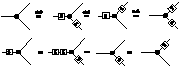
\includegraphics[width=0.6\textwidth]{Zstabs}\\
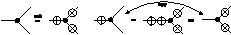
\includegraphics[width=0.650\textwidth]{Xstabs}\\
\includegraphics[width=0.50\textwidth]{XstabsYY}
\end{center}
\textit{(Top) Diagrammatic depiction of the stabilizer equation
$\sigma^z_i\sigma^z_j(\ket{000}+\ket{111})=\ket{000}+\ket{111}$. (Bottom)
Uses the stabilizer identity together with $\sigma_z^2=\I$ to show that
the $\sigma^z$ commutes with the black-dot. (Middle) Diagrammatic depiction of the stabilizer
equation
$\sigma^x_1\otimes\sigma^x_2\otimes\sigma^x_3(\ket{000}+\ket{111})=\ket{000
}+\ket{111}$.  (Bottom) Diagrammatic depiction (up to a sign) of the
stabilizer equation
$-\sigma^x_i\otimes\sigma^y_j\otimes\sigma^y_k(\ket{000}+\ket{111})=\ket{
000}+\ket{111}$.}
\end{example}
\end{comment}
%%%%%%%%%%%%%%%%%%%%%%%%%%%%%%%%%%%%%%%%%%

\begin{remark}[Gottesman-Knill Theorem] A
graphical rewrite proof (by bounding the number of rewrites) of the
Gottesman-Knill theorem follows by considering the action of the black and
plus dots on $\sigma^z$ and $\sigma^x$.  We will set proving this as an exercise in a later Lecture.  
\end{remark}

In addition to these two, one also finds the class of so called, \emph{symmetric states} (or operators for that matter). These are characterized as follows.  

\begin{example}[Invariance under $S_k$]
 The other form of symmetry that is considered, is invariance under the symmetric group.  Diagrammatically this amounts to braiding wires (where here the order of the braids is not relevant).  
\end{example}

We can relate symmetry in density operators and symmetry in states as follows.  
\begin{comment}
\begin{remark}[Symmetric density operators vs symmetric states]
A symmetric single qubit density operator necessarily has $bY=0$ and so gives rise to a symmetric two qubit state with real valued coefficients parametrized by two real degrees of freedom, $\psi_\rho(a, 0, c)$.  Diagrammaticality, a symmetric two-party state is invariant under exchange of it's legs whereas a symmetric density operator is invariant under exchange of its arms and legs (e.g. transpose).  
\begin{center}
 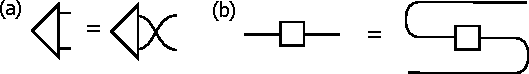
\includegraphics[width=10\xxxscale]{2-party-symmetric-states1}
\end{center}
\end{remark}
\end{comment}
\subsubsection*{Further symmetries of $\rho$.}  Now using these ideas, we can consider other symmetries of $\rho$.  We want to find solutions of 
\be 
\rho = V\rho V^\dagger 
\ee 
We will then consider 
\be 
\rho_\varepsilon' = a\I+ b\varepsilon 
\ee 
We then note that $b\in \7 R$ and that $\varepsilon = i Y$.  So we arrive at the density operator 
\be 
\rho_\varepsilon = a\I+ bY
\ee 
and will search for solutions to the equation 
\be 
\rho_\varepsilon = V\rho_\varepsilon V^\dagger = a V V^\dagger - b i V\varepsilon V^\dagger
\ee 
and note that under wire duality, 
\be
\varepsilon = S\varepsilon S^\top 
\ee 
(see Lemma \ref{lemma:epsilon-invariance}) and so $\rho_\varepsilon$ is invariant for 
\be 
V\in SU(n, \R)
\ee 
as those matrices satisfy $SS^\top=\I$.  We can go further however.  In fact, the following is easy to verify. 

\begin{lemma}[Isomorphism between projectors and self-adjoint unitary maps]
It is readily verified that 
\be 
 U = \I - 2P
 \ee 
 is unitary with $P^2=P$.  The equation is then solved for $P$ in terms of $U$.  
\end{lemma}
We then see that each projector gives rise to a symmetry of $\rho_\varepsilon$, as does the real orthogonal subgroup of the special unitary group.  





\section{Polynomial Invariants of Symmetric States}

A symmetric multipartite state or fully symmetric tensor carries the trivial representation of the symmetric group and hence is invariant under any permutation of the parties.  Examples are the three qubit
\GHZ-state $\ket{\text{\sf GHZ}} = \ket{000} +
\ket{111}$ and the three qubit W-state $\ket{\text{\sf W}} =
\ket{001} + \ket{010} + \ket{100}$. 

\begin{remark}[Symmetric basis]
A general $n$ qubit quantum system has the $2^n$ 
orthonormal basis vectors $\{ | 00 \dots 00 \rangle , | 00 \dots 01 \rangle , \dots , | 11 \dots 11 \rangle \}$. 
For the subspace of \emph{symmetric} $n$ qubit states, an orthonormal basis is given by 
the $n+1$ \emph{symmetric} basis states $\{ | S_{0} \rangle , | S_{1} \rangle , \dots , | S_{n} \rangle \}$. 
They are defined as
\begin{equation}
 \ket{S_{k}} = {\binom{n}{k}}^{- \frac{1}{2}} \sum_{\text{perm}}
\; \underbrace{ | 0 \rangle | 0 \rangle \cdots | 0 \rangle }_{n-k}
\underbrace{ | 1 \rangle | 1 \rangle \cdots | 1 \rangle }_{k}
\end{equation}
and called Dicke states.  We can therefore write $\ket{\text{\sf W}} = \ket{{S}_{1}}$ and $\ket{\text{\sf GHZ}} =
\frac{1}{\sqrt{2}} ( \ket{{S}_{0}} + \ket{{S}_{3}})$.
\end{remark}


\begin{myexercise}[Boolean symmetric states]
 Provide the number of symmetric Boolean quantum states.  
\end{myexercise}


\paragraph{A polynomial basis.}
Symmetric qubit states and symmetric polynomials in two variables are isomorphic as vector spaces.  The known mapping is accomplished as follows.  
\begin{equation}
 \ket{0} \leftrightarrow x, ~~~~~~~~~~ \ket{1}\leftrightarrow  y
\end{equation}

\begin{remark}[Creation and annihilation operators]
 If we consider a symmetric polynomial basis in $x^n$, we can define two operators
 \be 
 a^+ : = x
 \ee 
 \be 
 a^- := \frac{\partial}{\partial x} := \partial_x
 \ee 
 From this we can define an inner product on our space.  For instance, we 
 can calculate the norm of $x^n$ as 
 \be 
 \braket{x^n}{x^n}= \braket{x^n}{a^+ x^{n-1}} = \braket{a^- x^n}{x^{n-1}} = n! 
 \ee 
 This concept is readily extended to the case of binary forms in $x$ and $y$ when considering creation and annihilation operators for each variable $x$ and $y$ separately.  
\end{remark}

\begin{example}[Polynomials for the \GHZ-class]
The $n$-partite GHZ state $\ket{0}^{\otimes n}+\ket{1}^{\otimes n}$ 
has homogeneous polynomial $f(x,y)=x^n+y^n$.
\end{example}

\begin{example}[Polynomials corresponding to common quantum states]
The three-qubit W state
$\ket{W_3}=\ket{001}+\ket{010}+\ket{100}$ is isomorphic to the
monomial $3x^2 y$. Furthermore, two appropriately braided copies of $\ket{W_3}$ read 
$\ket{W_{3,3}}=(\ket{003}+\ket{030}+\ket{300})+(\ket{012}+\ket{021}+\ket{102}+\ket{120}+\ket{201}+\ket{210})$ which is given diagrammatically as 
\begin{center}
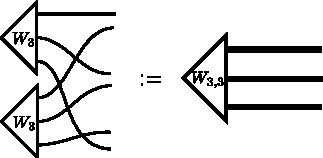
\includegraphics[width=6\xxxscale]{W-states}
%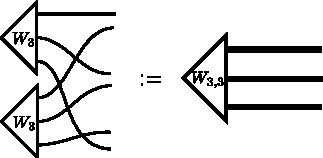
\epsfig{figure=W-states,width=6cm}  
\end{center}
and becomes a sum of two Dicke states having corresponding homogeneous
polynomials $x_0^2 x_3$ and $x_0x_1x_2$. It is isomorphic to the
homogeneous polynomial $3x_0^2 x_3+6x_0x_1x_2$. 
\end{example}

It turns out that the invariant theory of binary forms is well studied in the literature.  An invariant of a binary form is a polynomial in the coefficients of a binary form in two variables $x$ and $y$ that remains invariant under invertible transformations of the variables $x$ and $y$.  

 
\section*{Invariants of forms} 

\begin{example}
 Consider 
 \be 
 ax^2 + 2bx + c = 0
 \ee 
 where the discriminant is 
 \be 
 \Delta = b^2 - ac
 \ee 
 If $\Delta = 0$ we have a double root, and if $\Delta < 0$ the roots are complex conjugate.  Now if we consider the affine change of variables, where $\alpha \neq 0$ 
 \be 
 x' = \alpha x + \beta 
 \ee 
Upon calculating the discriminant for the polynomial in the new variables we arrive at 
\be 
\Delta' = \frac{1}{\alpha^2} \Delta
\ee 
which is the same as $\Delta$ in the original polynomial, up to a multiplicative factor that depends only on the transformation.  The properties of the roots remain unchanged under such transformations.  
\end{example}

\section{From Binary Forms to Qubit States} 

We will now consider our subject of interest.  Forms in two variables, called quadratic forms, or binary forms.  
For example, the general degree two binary form is given as  
\be 
Q(x,y) = a_2 x^2 + 2 a_1 xy + a_0 y^2
\ee 
which gives rise to the quantum state 
\be 
\psi_Q = a_2\ket{00} + a_1 (\ket{01}+\ket{10}) + a_0 \ket{11}
\ee 

\begin{definition}[General linear invertible transformation]
 A general linear invertible transformation of two variables takes the form 
 \be 
 x' = \alpha x + \beta y
 \ee 
 \be 
 y' = \gamma x + \delta y
 \ee 
 where 
 \be 
 \alpha \delta - \beta \gamma \neq 0
 \ee 
 When a variable is transformed, we get an induced transformation of the coefficients.  It is important to note that this transformation does not change the degree of a given polynomial.  
\end{definition}

\begin{definition}[Invariant of a binary form \cite{oliver}]
 An invariant of a binary form $Q(x,y)$ is a function $I(a) = I(a_0, ..., a_1)$ depending on the coefficients 
 $a= (a_0, ..., a_n)$ of the form, which, up to a determinantal factor, does not change under the general linear 
 transformation 
 \be 
 I(a) = (\alpha \delta - \beta \gamma)^k I(a')
 \ee 
 where $a' = (a_0', ..., a_n')$ are the transformed coefficients.  
\end{definition}

An integer $k$ is called the weight of the invariant and we are concerned with the case that $I(a)$ is a polynomial.  
It is then called, a polynomial invariant.  

\begin{remark}
 Classical invariant theory has provided us elegant solutions to the following questions \cite{hilbert, oliver}.  
 \begin{itemize}
  \item[(i)] How many independent polynomial invariants are there of a given degree?
  \item[(ii)] What do they tell us about the form? 
  \item[(iii)] Can we find a basis for the polynomial invariants? 
 \end{itemize}
\end{remark}

We are missing an important piece to our puzzle.  These are the covariants, which are polynomials.  

\begin{definition}[Covariant \cite{oliver}]
 A covariant of weight $k$ of a binary from $Q$ of degree $n$ is a function 
 \be 
 J(a, x, y)
 \ee 
 depending both on the coefficients $a_i$ and on the independent variables $(x,y)$ which up to a determinantal factor, in unchanged under general linear transformations 
 \be 
 J(a, x, y) =  (\alpha \delta - \beta \gamma)^k J'(a', x', y')
 \ee 
\end{definition}


% \section*{Two qubits}
 

\section*{Three qubit example} 
The cubic binary form is given as 
\be 
Q(x,y) = a_3 x^3 + 3 a_2 x^2y + 3 a_1 xy^2 + a_0 y^3
\ee 
It is known that there is just one fundamental invariant, the discriminant of the cubic.
\be 
\Delta = a_0^2 a_3^2 - 6 a_0 a_1 a_2 a_3 + 4 a_0 a_2^3 - 3a_1^2 a_2^2 + 4 a_1^3 a_3
\ee 

\begin{remark}
 $\Delta = 0$ iff $Q$ has a double or triple root.  
\end{remark}


\begin{myexercise}
 Consider the discriminant of the cubic.
\be 
\Delta = a_0^2 a_3^2 - 6 a_0 a_1 a_2 a_3 + 4 a_0 a_2^3 - 3a_1^2 a_2^2 + 4 a_1^3 a_3
\ee 
and find maximum and minimum values when $\forall i, a_i\in \{0,1\}$. 
\end{myexercise}


The obvious covariant is the form itself.  Another important covariant is the Hessian 
\be 
H = Q_{xx}Q_{yy} - Q_{xy}^2
\ee 
where we use subscripts to denote partial derivatives.  
For the binary cubic, the Hessian becomes 
\be 
\frac{1}{36} H = (a_1a_3 - a_2)x^2 + (a_0 a_3 - a_1 a_2)xy + (a_0a_2 - a_1^2)y^2 
\ee 

\begin{theorem}[vanishing Hessian \cite{oliver}]
 A binary form $Q(x,y)$ has vanishing Hessian, $H=0$ iff $Q(x,y)= (cx+dy)^n$, that is iff $Q(x,y)$ is the nth power of a linear form.  
\end{theorem}

\begin{remark}[Applications to quantum entanglement]
 It is clear that a linear form 
 \be 
 Q(x,y)= (cx+dy)^n
 \ee 
 gives rise to a factorisable quantum state as 
 \be 
 \psi_Q = (c\ket{0}+ d\ket{1})^n
 \ee 
 So clearly, the Hessian corresponding to a quantum state, determines if the state can be written as a local product of 
 operators.  Other covariants give additional information. 
 
%  Given values of $H$ and $\Delta$, we can already conclude the following about a given state.  
%  
%  \begin{center}
% \begin{tabular}{c||c||c||c}
% (i)    & $\Delta\neq 0$        & simple roots & non-separable\\
% (ii)   & $\Delta=0$, $H\neq=0$ & × & ×\\
% (iii)  & $H=0$ & × & ×
%  \end{tabular}
%  \end{center}

\end{remark}




\begin{remark}[Sylvester's tables]
In the mid 1800s Sylvester produced tables\marginnote{{\it ``The object of pure physics is the unfolding of the laws of the intelligible world; the object of pure mathematics that of unfolding the laws of human intelligence.''} --- James Joseph Sylvester.} predicting numbers of invariants and covariants of a given degree.  The table should only be trusted for covariants up to degree 6 and invariants up to degree 8.  
 \begin{center}
\begin{tabular}{c||cccccccccc}
\hline
degree     & 2 & 3 & 4 & 5 & 6 & 7 & 8 & 9 & 10 & 12 \\\hline \hline 
invariants & 1 & 1 & 2 & 4 & 5 & 26 (30) & 9 & 89 & 104 & 109 \\
covariants & 2 & 4 & 5 & 23 & 26 & 124 (130) & 69 & 415 & 475 & 947 \\\hline 
\end{tabular}
\end{center}
\end{remark}

\section{Problems} 

\subsection*{Anti-linear operators} 

\begin{remark}
Tensor contraction is linear.  Tensor networks encapsulate multilinear algebra.  What about antilinear operators or non-linear operators (such as those found in tensor flow software)?  As a prelude, let us first consider some properties of antilinear operators.  Readers should first show that complex conjugate is antilinear. 
\end{remark}

\begin{definition}[Qubit density operator]
Consider a density operator of a single spin (a.k.a.~qubit) as
\begin{equation}
\rho = \frac{1}{2}(\I + a.\sigma)
\end{equation}
where $a=(a^1, a^2, a^3)\in [-1,1]^{\otimes 3}\subset \mathbb{R}^3$, the Pauli vector $\sigma=(\sigma_1, \sigma_2, \sigma_3) = (X, Y, Z)$ and `.' signifies a sum over the entry wise product, viz.~$a.\sigma = \sum_i a^i \sigma_i$.  Here $\Tr \rho = 1$, $\rho \geq 0$, $\rho=\rho^\dagger$, $\sum_{i\in\{1,2,3\}} |a^i|\leq 1$ (the vector $a$ also satisfies $||a||_2\leq 1$). 
\end{definition}
  
\begin{definition}[T-action]\label{def:taction}
For the polarization vector $\sigma$, we define $T$ through the action $T\sigma T^\dagger = - \sigma$. 
\end{definition}

\begin{myexercise}
Prove that $T$ as defined in \ref{def:taction} is not unitary.  (Hint consider preservation of the definition of the Pauli-algebra under unitary group homomorphism). 
\end{myexercise}

\begin{myexercise}
Show that $\prod_{i=1, 2, 3}\Tr \sigma_i \rho = a_1a_2a_3$.  
\end{myexercise}

We will consider the form of $T=UK$ where $U$ is unitary and $K$ is complex conjugation.

\begin{myexercise}
For a single qubit, let $T = e^{-\imath \frac{\pi}{2} Y}K$ and  show  that this definition satisfies the definition of the T-reversal operator from \ref{def:taction}. 
\end{myexercise}

\begin{myexercise} Show that 
$[\rho, T]=0$ for $T = e^{-\imath \frac{\pi}{2} Y}K$ iff $\rho = \frac{1}{2}\I$. 
\end{myexercise}

\begin{myexercise}
Show that $[\rho, K]=0$ iff $a_2=0$, in which case $T\sim Y$.\footnote{$\sim$ denotes equality up to an equivalency class defined by  unit norm complex numbers.}
\end{myexercise}

\begin{remark}[Dagger of qubit maps]
Let us write the general local qubit map, using the following
parameterization which can express any single-qubit map. 
\be 
U(2,\7C) = U(1, \7C)\times SU(2, \7C) 
\ee 
so up to a negligible global phase, every local unitary map on qubits is
effectively given by a special unitary map. Consider then, 
\be 
S = \alpha\ketbra{0}{0} - \overline{\beta}\ketbra{0}{1} + \beta
\ketbra{1}{0} + \overline{\alpha}\ketbra{1}{1}. 
\ee 
It is a straight forward calculation to verify that 
\be 
[\epsilon^\top S \epsilon]^\top = S^\dagger. 
\ee
Which has the diagrammatic form as: 
 \begin{center}
 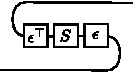
\includegraphics[width=0.25\textwidth]{dagger-by-epsilon} 
\end{center}
\end{remark}





% \paragraph{The dagger is linear on qubit maps.}  We have mentioned a
% somewhat surprising fact during this course.  That is, the dagger of a map,
% the conjugate transpose, can be given by a linear operation for the case of
% qubit maps.  To begin with, let us recall that 
% \be 
% U(2,\7C) = U(1, \7C)\times SU(2, \7C) 
% \ee 
% so up to a negligible global phase, every local unitary map on qubits is
% effectively given by a special unitary map.  The determinate of a general
% unitary map is given by a complex number, whereas the determinate of a
% special unitary map is always one.  

% \begin{theorem}[Linearity of the dagger for qubit maps]
% The dagger of any quantum circuit, inducing a map $C$ acting on qubits,
% built from \CNOT-gates, and arbitrary local special unitary rotations is
% linear, up to a negligible global phase factor. 

% \begin{proof}[Linearity of the dagger for qubit maps]
% Let us write the general local qubit map, using the following
% parameterization which can express any single-qubit map.  
% \be 
% S = \alpha\ketbra{0}{0} - \overline{\beta}\ketbra{0}{1} + \beta
% \ketbra{1}{0} + \overline{\alpha}\ketbra{1}{1}
% \ee 
% It is a straight forward calculation to verify that 
% \be 
% [\epsilon^\top S \epsilon]^\top = S^\dagger 
% \ee
% Which has the diagrammatic form as.  
%  \begin{center}
%  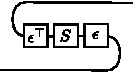
\includegraphics[width=0.25\textwidth]{dagger-by-epsilon} 
% \end{center}
% Now from the fact that \CNOT$^2=\I$ we simply reverse the order of the
% gates in the circuit $C$, replacing each local gate $S$ with
% $[\epsilon^\top S \epsilon]^\top = S^\dagger$ leading directly to
% $C^\dagger$.  We note that $\epsilon = ZX$ and $\epsilon^\top =
% XZ=-\epsilon$.  
% \end{proof}
% \end{theorem}

